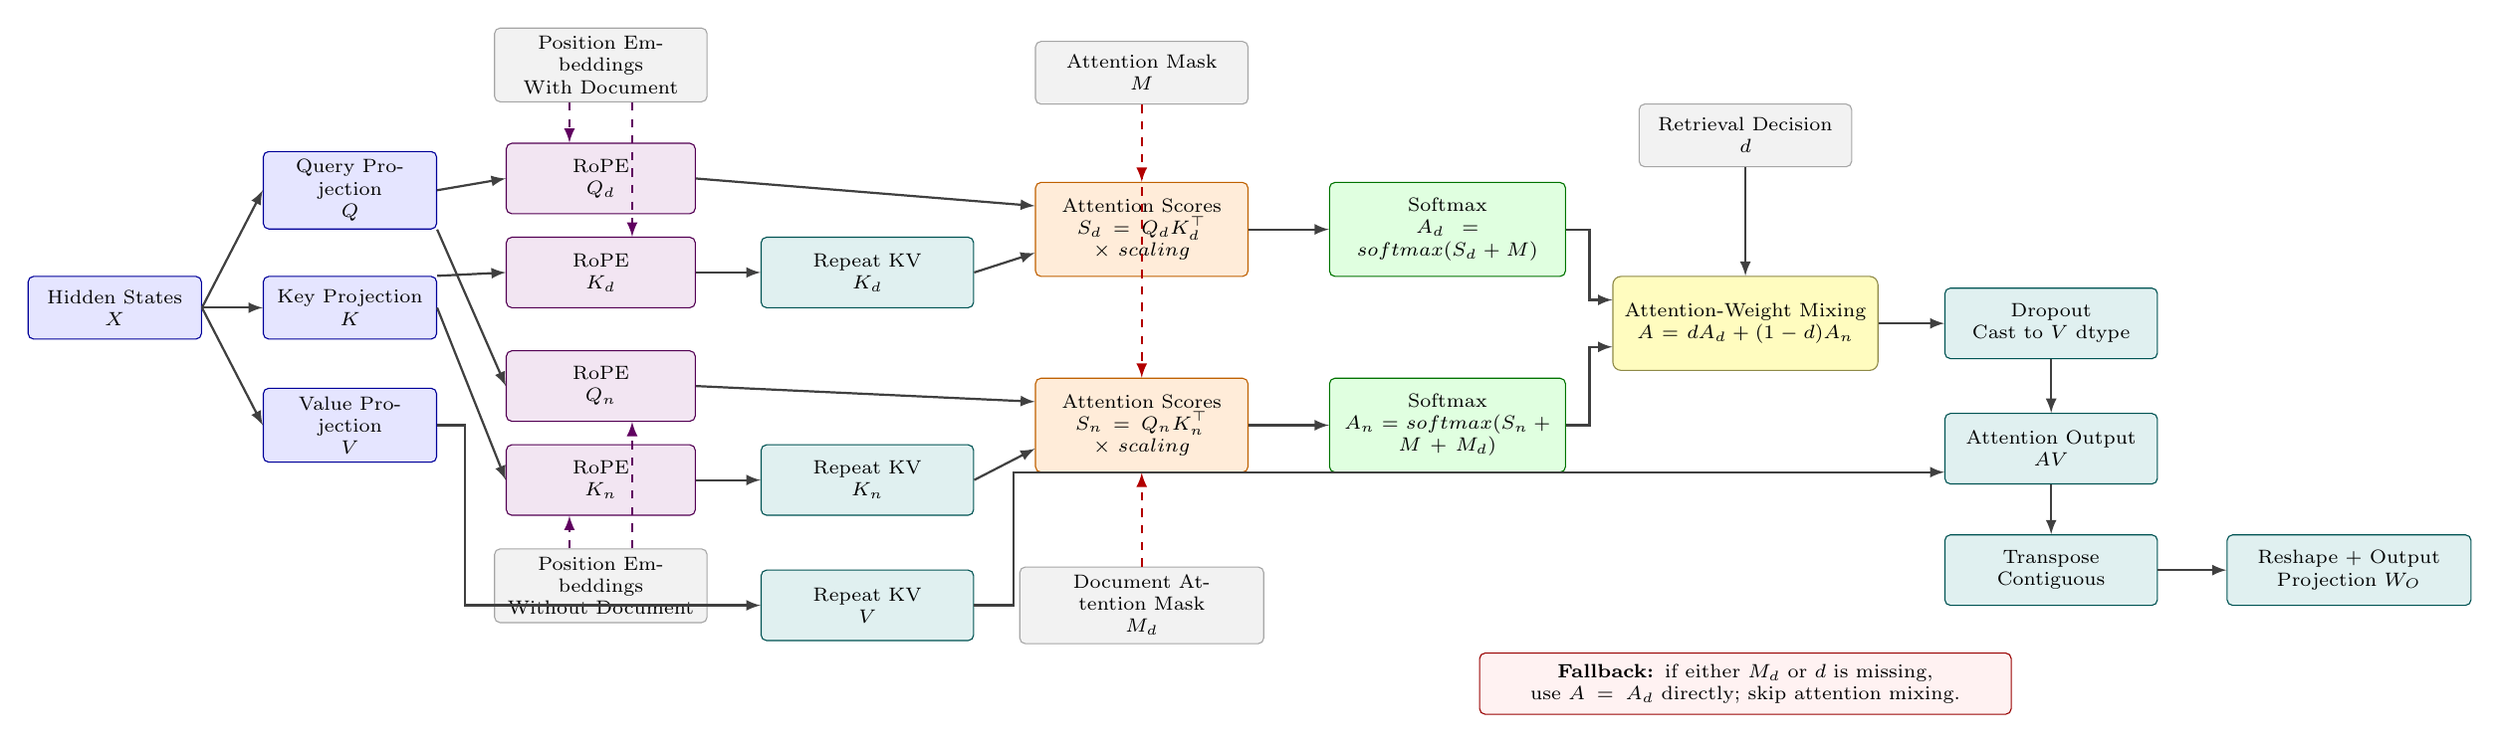
\begin{tikzpicture}[
    font=\scriptsize,
    >=latex,
    input/.style={
        draw=blue!60!black,
        fill=blue!10,
        rounded corners=2pt,
        align=center,
        minimum height=8mm,
        text width=20mm,
        inner sep=3pt
    },
    rope/.style={
        draw=violet!65!black,
        fill=violet!10,
        rounded corners=2pt,
        align=center,
        text width=22mm,
        minimum height=9mm,
        inner sep=3pt
    },
    score/.style={
        draw=orange!75!black,
        fill=orange!15,
        rounded corners=2pt,
        align=center,
        text width=25mm,
        minimum height=12mm,
        inner sep=3pt
    },
    softmax/.style={
        draw=green!45!black,
        fill=green!12,
        rounded corners=2pt,
        align=center,
        text width=28mm,
        minimum height=12mm,
        inner sep=3pt
    },
    mix/.style={
        draw=yellow!50!black,
        fill=yellow!25,
        rounded corners=3pt,
        align=center,
        text width=31mm,
        minimum height=12mm,
        inner sep=4pt
    },
    output/.style={
        draw=teal!65!black,
        fill=teal!12,
        rounded corners=2pt,
        align=center,
        text width=25mm,
        minimum height=9mm,
        inner sep=3pt
    },
    auxiliary/.style={
        draw=gray!70,
        fill=gray!10,
        rounded corners=2pt,
        align=center,
        text width=25mm,
        minimum height=8mm,
        inner sep=3pt
    },
    arrow/.style={->, thick, draw=black!75},
    posarrow/.style={->, thick, dashed, draw=violet!75!black},
    maskarrow/.style={->, thick, dashed, draw=red!70!black}
]

% =========================================================
% 1. INPUT AND Q/K/V PROJECTIONS
% =========================================================

\node[input] (hidden) at (0,0)
    {Hidden States\\$X$};

\node[input] (qproj) at (3,1.5)
    {Query Projection\\$Q$};

\node[input] (kproj) at (3,0)
    {Key Projection\\$K$};

\node[input] (vproj) at (3,-1.5)
    {Value Projection\\$V$};

\draw[arrow] (hidden.east) -- (qproj.west);
\draw[arrow] (hidden.east) -- (kproj.west);
\draw[arrow] (hidden.east) -- (vproj.west);

% =========================================================
% 2. RoPE: TWO POSITION-EMBEDDING PATHS
% =========================================================

\node[auxiliary] (posdoc) at (6.2,3.1)
    {Position Embeddings\\With Document};

\node[rope] (qdoc) at (6.2,1.65)
    {RoPE\\$Q_d$};

\node[rope] (kdoc) at (6.2,0.45)
    {RoPE\\$K_d$};

\node[rope] (qnodoc) at (6.2,-1.0)
    {RoPE\\$Q_n$};

\node[rope] (knodoc) at (6.2,-2.2)
    {RoPE\\$K_n$};

\node[auxiliary] (posnodoc) at (6.2,-3.55)
    {Position Embeddings\\Without Document};

% Q branches: diagonal arrows
\draw[arrow] (qproj.east) -- (qdoc.west);
\draw[arrow] (qproj.south east) -- (qnodoc.west);

% K branches: diagonal arrows
\draw[arrow] (kproj.north east) -- (kdoc.west);
\draw[arrow] (kproj.east) -- (knodoc.west);

% Position Embeddings -> RoPE
% Straight vertical dashed arrows, slightly separated horizontally

% With Document
\draw[posarrow]
    ([xshift=-4mm]posdoc.south)
    -- ([xshift=-4mm]qdoc.north);

\draw[posarrow]
    ([xshift=4mm]posdoc.south)
    -- ([xshift=4mm]kdoc.north);

% Without Document
\draw[posarrow]
    ([xshift=-4mm]posnodoc.north)
    -- ([xshift=-4mm]knodoc.south);

\draw[posarrow]
    ([xshift=4mm]posnodoc.north)
    -- ([xshift=4mm]qnodoc.south);

% =========================================================
% 3. REPEAT KV HEADS
% =========================================================

\node[output] (repeatkd) at (9.6,0.45)
    {Repeat KV\\$K_d$};

\node[output] (repeatkn) at (9.6,-2.2)
    {Repeat KV\\$K_n$};

\node[output] (repeatv) at (9.6,-3.8)
    {Repeat KV\\$V$};

\draw[arrow] (kdoc.east) -- (repeatkd.west);
\draw[arrow] (knodoc.east) -- (repeatkn.west);
\draw[arrow] (vproj.east) -- ++(0.35,0) |- (repeatv.west);

% =========================================================
% 4. ATTENTION SCORES
% =========================================================

\node[score] (scoresd) at (13.1,1.0)
    {Attention Scores\\
     $S_d=Q_dK_d^\top$\\
     $\times\ \text{scaling}$};

\node[score] (scoresn) at (13.1,-1.5)
    {Attention Scores\\
     $S_n=Q_nK_n^\top$\\
     $\times\ \text{scaling}$};

% Q and K enter at separated points on the score nodes
\draw[arrow] (qdoc.east)
    -- ([yshift=3mm]scoresd.west);

\draw[arrow] (repeatkd.east)
    -- ([yshift=-3mm]scoresd.west);

\draw[arrow] (qnodoc.east)
    -- ([yshift=3mm]scoresn.west);

\draw[arrow] (repeatkn.east)
    -- ([yshift=-3mm]scoresn.west);

% =========================================================
% 5. MASKS AND SOFTMAX
% =========================================================

\node[auxiliary] (causal) at (13.1,3.0)
    {Attention Mask\\$M$};

\node[auxiliary, text width=29mm] (docmask) at (13.1,-3.8)
    {Document Attention Mask\\$M_d$};

\node[softmax] (softd) at (17.0,1.0)
    {Softmax\\
     $A_d=\operatorname{softmax}(S_d+M)$};

\node[softmax] (softn) at (17.0,-1.5)
    {Softmax\\
     $A_n=\operatorname{softmax}(S_n+M+M_d)$};

\draw[arrow] (scoresd.east) -- (softd.west);
\draw[arrow] (scoresn.east) -- (softn.west);

% Attention mask is added to both score tensors
\draw[maskarrow]
    (causal.south) -- ++(0,-0.2) -| (scoresd.north);

\draw[maskarrow]
    (causal.south) -- ++(0,-0.4) -| (scoresn.north);

% Document mask is added only to the without-document scores
\draw[maskarrow]
    (docmask.north) -- ++(0,0.2) -| (scoresn.south);

% =========================================================
% 6. RETRIEVAL DECISION AND ATTENTION MIXING
% =========================================================

\node[auxiliary] (decision) at (20.8,2.2)
    {Retrieval Decision\\$d$};

\node[mix] (mix) at (20.8,-0.2)
    {Attention-Weight Mixing\\
     $A=dA_d+(1-d)A_n$};

\draw[arrow] (softd.east) -- ++(0.3,0) |-
    ([yshift=3mm]mix.west);

\draw[arrow] (softn.east) -- ++(0.3,0) |-
    ([yshift=-3mm]mix.west);

\draw[arrow] (decision.south) -- (mix.north);

% =========================================================
% 7. DROPOUT, ATTENTION OUTPUT, AND PROJECTION
% =========================================================

\node[output] (dropout) at (24.7,-0.2)
    {Dropout\\Cast to $V$ dtype};

\node[output] (attnout) at (24.7,-1.8)
    {Attention Output\\$A V$};

\node[output] (transpose) at (24.7,-3.35)
    {Transpose\\Contiguous};

\node[output, text width=29mm] (outproj) at (28.5,-3.35)
    {Reshape + Output\\Projection $W_O$};

\draw[arrow] (mix.east) -- (dropout.west);
\draw[arrow] (dropout.south) -- (attnout.north);

% Shared V path enters Attention Output
\draw[arrow] (repeatv.east) -- ++(0.5,0) |-
    ([yshift=-3mm]attnout.west);

\draw[arrow] (attnout.south) -- (transpose.north);
\draw[arrow] (transpose.east) -- (outproj.west);

% =========================================================
% 8. FALLBACK BEHAVIOUR
% =========================================================

\node[
    draw=red!60!black,
    fill=red!5,
    rounded corners=2pt,
    align=center,
    text width=65mm,
    inner sep=4pt
] (fallback) at (20.8,-4.8)
    {\textbf{Fallback:} if either $M_d$ or $d$ is missing,\\
     use $A=A_d$ directly; skip attention mixing.};

\end{tikzpicture}